\documentclass[12pt]{article}

\usepackage{enumitem}
\usepackage[right=20mm, left=20mm]{geometry}
\usepackage{type1cm}
\usepackage{amssymb}
\usepackage[fleqn]{amsmath}
\usepackage{tikz}
\usepackage{multicol}
\usepackage{makecell}
\setlength{\columnsep}{1pt}
\usepackage{pgfplots}
\usepackage{float}
\usepackage{caption}
\usepackage{subcaption}
% \usepackage{subfig}
\usepackage{graphicx}

\usepackage{indentfirst}
\usepackage{lastpage}  
\usepackage{fancyhdr}
\pagestyle{fancy}

\usepackage[unicode=true,pdfusetitle,
 bookmarks=true,bookmarksnumbered=false,bookmarksopen=false,
 breaklinks=false,pdfborder={0 0 1},backref=false,colorlinks=false]
 {hyperref}

\makeatletter
\newenvironment{myalign*}{\ifvmode\else\hfil\null\linebreak\fi
  \hspace*{-\leftmargin}\minipage\textwidth
  \setlength{\abovedisplayskip}{0pt}%
  \setlength{\abovedisplayshortskip}{\abovedisplayskip}%
  \start@align\@ne\st@rredtrue\m@ne}%
{\endalign\endminipage\linebreak}

% Paper size
\topmargin -10mm
\textwidth 170mm
% \oddsidemargin -5mm
% \evensidemargin -5mm
\textheight 220mm

% Font setting
\usepackage{xeCJK}
% \setCJKmainfont{Noto Sans TC}
\setCJKmainfont{kaiu.ttf}


\renewcommand{\footnotesize}{\normalsize} 
\renewcommand{\headrulewidth}{0pt}
\renewcommand{\footrulewidth}{0pt}

\lhead{}
\chead{整合式線上教學平台ProgLearn}
\rhead{}

\lfoot{}
\cfoot{}
\rfoot{ 共 \pageref{LastPage} 頁 第  \thepage   頁} 

\makeatletter
\begin{document}
% \fontsize{14pt}{18pt}\selectfont
% \author{}
\date{}
\usetikzlibrary{automata, positioning, arrows}
% \maketitle
\tikzset{every state, accepting/.style={double distance=2pt}}
\captionsetup[figure]{labelfont={bf},name={圖},labelsep=period}

\begin{enumerate}
  \setlength{\parindent}{2em}
  \item 摘要 
    \par 本計畫將建立一個專注於教師導向的教學工具,
    名為 ProgLearn ,這個整合式教學平台將提供課堂教學系統和線上解題系統(OJ, Online Judge)
    $\footnote{線上解題系統:演算法競賽中,用以評測程式碼正確性的系統,可用於練習、求職面試以及競賽。}$。
    課堂教學系統將包含影音、互動式講義以及課堂練習。

    影音將提供同步和非同步教學,而互動式講義不再是傳統的圖像及文字,
    將使用 JS (JavaScript) 技術製作,以增加學生和教師的互動。
    OJ 將包含傳統的題目撰寫外,還提供自動反饋錯誤訊息的功能,
    並且可以分析學生提交的程式碼,以提高學生的學習效果。

    課堂練習平台將採用 OJ 模組,如果採用同步教學,
    學生提交的程式碼可以即時在課堂練習上呈現,讓教師和學生可以即時互相評論與回饋。

    除此之外, ProgLearn 系統還將提供可自訂的測試案例,以方便教師進行練習的設計。
    綜上所述, ProgLearn 是一個結合教學與練習的完整教學平台,旨在提高學生的學習效率,
    並改善教師的教學效率。

  \item 研究動機與研究問題
    \par 在台灣,資訊科技領域受到廣泛重視。
    根據十二年國民基本教育課程綱要\cite{ref2},
    程式設計已被列為學校必修課程,每年有數百萬學生修習程式教育\cite{ref3}。
    然而,在基層教育中卻存在許多問題:
    \begin{enumerate}
      \setlength{\parindent}{2em}
      \item 教師在教學與備課的工作量大:
        \par 比如準備線上課程的直播環境、準備課程教材、批改學生作業、
        上傳考題、課外時間回覆學生的各種問題等\cite{ref4}。
        由於專業教師與學生數量的比例失衡,也讓教師難以管理學生\cite{ref5}。
      \item 受技術限制的教學方式:
        \begin{itemize}
          \item 線下課程:資訊教室大多使用資訊教室的廣播與管理系統
          $\footnote{資訊教室的廣播與管理系統:針對資訊教室的廣播與管理系統,可將電腦畫面傳送給特定或所有使用者端,並且能監控使用者端的電腦畫面。}$
          ,讓教師能夠強制監控所有學生的電腦,並在課堂中分享自己的畫面。
          雖然這種方式能讓學生專注於教師的授課中,但強制控制學生的電腦,
          學生就無法在上課過程中使用顯示畫面以外的電腦功能,如查詢資料、閱讀過往的課程講義、實作程式碼等,
          大大限制學生的學習空間。
          \item 線上課程:教師的教學設備品質,會影響學生學習情緒及上課意願\cite{ref7}。
          此外,線上自主學習,學生若有問題無法獲得即時解答,學習效果可能受限\cite{ref4}。
        \end{itemize}
      \item 師生間缺乏互動性:
        \begin{itemize}
          \item 線下課程:資訊教室要實現師生間的雙向互動,大多以麥克風作為訊息傳遞的媒介,
          但對於有限的麥克風數量、有限的教室空間,增加教師教學的難度。
          \item 線上課程:教師大多以直播軟體搭配投影音教學,由於缺乏實際互動,
          難以保持學生的學習熱忱,並且教師無法即時注意學生的反應而影響其教學成效\cite{ref7}。
          並且透過軟體建置的網路平台,並非只能以影音、圖文作為訊息的傳遞方式,比如 youtube 的 Crowd Choice 功能$\footnote{https://support.google.com/youtube/answer/9955116?hl=zh-Hant}$
           、 youtube 直播時的即時問答功能$\footnote{https://youtu.be/XdfdwqPgL3I}$、 HackMD$\footnote{https://hackmd.io}$ 的線上共筆功能、 Twitch 實況互動元件$\footnote{https://www.twitch.tv/p/zh-tw/extensions/}$等,
          都是可以被利用的互動性功能。教師應提供好的遠距教學平台與工具,增進師生互動\cite{ref4}。
        \end{itemize}
      \item 教學工具種類繁多且功能單一:
        \begin{itemize}
          \item 線下課程:教師在課堂中常使用資訊教室的廣播與管理系統搭配投影音。
          課後作業則以紙本與程式解題系統,如高中生程式解題系統$\footnote{https://zerojudge.tw/}$、
           iTSA 程式自學平臺$\footnote{https://e-tutor.itsa.org.tw/e-Tutor/}$等。
          同一堂課,師生必須同時使用多種軟體與網站。
          \item 線上課程:為因應 COVID-19 的疫情,以網路同步直播教學為主,
          許多基層教師利用 Google Meet $\footnote{https://meet.google.com/}$
          或 Microsoft Teams $\footnote{https://www.microsoft.com/zh-tw/microsoft-teams/}$
          等軟體進行線上同步直播教學,然而,這些軟體並不是針對教學而設計的,
          如作業的批改、實作、課程內容的簡報、回顧等,仍需要使用其他軟體。
          \item 共同問題:缺乏整合的教學空間,導致學生和教師因教學系統過於複雜而不易使用。
        \end{itemize}
    \end{enumerate}
    \par 基於以上問題,本計畫旨在通過改進教學方式,幫助教師以最小的成本實現預期的教學效果,從而提高學生的學習體驗和效果。
    
    \par 市面上的線上教學平台,如均一教育平台$\footnote{https://www.junyiacademy.org/}$
    、 Microsoft Learn $\footnote{https://learn.microsoft.com/zh-tw/}$
    、 Hahow好學校 $\footnote{https://hahow.in/}$,
    主要通過靜態圖文與非同步影音的方式提供教學內容,缺乏學生和教師之間的互動。
    然而,這種教學模式存在許多問題,例如:教師只負責提供教學內容,學生需自主完成課題;
    缺乏教師的即時指導和回饋,導致學生的學習動機不高;
    教師無法從學生的學習過程中得到反饋,無法衡量教學效果\cite{ref4}。
    
    \par 目前的線下實體教學,大多使用資訊教室的廣播與管理系統強制監控學生的電腦,這導致許多問題:
    學生無法在授課過程中及時吸收與實作;當教師將電腦控制權交還給學生時,學生可能無法跟上進度;
    課程講義需要學生自行下載並換頁,教師還需要暫停授課以給學生練習的時間。
    綜上所述,缺乏互動性和靈活性是造成這些問題的原因。
    因此,我們需要一個更先進、更符合現代教育需求的教學平台。

    \par 這個平台應該具有以下特點:
    方便學生在課堂上隨時參與實作,提供靈活的控制功能,讓教師能夠輕鬆地調整課程進度,並具有清晰易懂的講義介面。
    這樣的教學平台不僅可以幫助學生更好地吸收知識,還能提高教師的教學效率和效果。
    
    \par 此外,當專業教師缺乏時,教師無法完全關注學生的學習情況。
    透過自然語言 AI 的協助,學生可以隨時提出問題並得到回覆與建議。將其運用於課堂和作業批改中,可以大幅減低教師的教學壓力。
    
    \par 本計畫預計將開發一個名為 Proglearn 的 Web 應用系統,教師將是主要使用者。該平台提供兩個模組,教學模組和題目練習模組。
    教學模組將允許教師創建多個班級,每個班級也可以有多個教師。
    教師可以在一個班級中創建多個課程,這些課程將包含影音、投影片、課堂練習、作業等。影音將會有同步的和非同步兩種形式。
    同步影音將使用低延遲直播技術,可以是電腦螢幕直播,也可以是人像直播或同時進行。
    非同步視頻將由教師上傳教學影音。
    教學簡報將使用 JS 生成,允許教師直接控制簡報並與影音互動。
    課程練習的題目將由教師從題目練習模組中選擇。
    在同步影音教學過程中,學生的程式碼或答案可以被分析,並將結果同步給教師,以便對學生的學習進度進行更及時的評估。
    而作業類似於課堂練習,允許學生在課後進行練習。這些作業的結果也可以被分析出來,並且可以讓教師更快速的追蹤學生的練習情況。
    題目練習模組是一個線上練習題系統,教師可以在這裡添加問題,並支持使用 ICPC problem package$\footnote{https://icpc.io/problem-package-format/}$ 添加新問題。
    本系統超越了傳統的 OJ ,增加了程式碼分析等功能。
    如果學生提交的程式碼有錯誤,人工智慧會及時向學生提供反饋。
    \par 通過這種方式, Proglearn 為教師提供了一個全面的教學平台,以改善學生的學習體驗和表現。

  \item 文獻回顧與探討
    \par 以下文獻回顧針對本計畫之背景知識進行分析與探討,從應用的各項功能設計與使用者的教學需求分析,
    其中包含低延遲直播技術、教學功能的需求與成效分析、自動反饋與程式碼分析技術。
    \begin{enumerate}
      \setlength{\parindent}{2em}
      \item 低延遲直播技術
        \par 此研究旨在開發一個低延遲的同步教學平台。
        這個平台將支持分享電腦螢幕和人像直播功能。
        市面上常見的視訊串流直播技術: RTMP (Real-Time Messaging Protocol) 、
         HLS (HTTP Live Streaming) 、
         DRM (Digital Rights Management) 、
         WebRTC (Web Real-Time Communication) 。
         RTMP 技術長用於線上遊戲和多人直播。
         HLS 是使用 HTTP 協議,在不同的網絡環境中提供高質量的實時串流。
         DRM 技術用於保護數位內容,通常用於付費串流平台中,以防止內容被盜。
        而 WebRTC 是一個用於即時通信的方案,如解題直播等需要高互動性的情景。
        \par 在 Ouya %Samuel Ouya
        等作者的論文中\cite{ref13},作者探討了使用 WebRTC 技術來實現遠端教育的平台。
         WebRTC 是 google 的一個開源項目,用於網絡瀏覽器之間的實時通信。
        它使用一個 JS API ,直接在瀏覽器中實現視訊通話、文件傳輸、 P2P 訊息分享和其他功能,而不需要額外的插件或程式。
        憑藉其現代軟體技術,如資料通道和串流傳輸, WebRTC 提供了一個高效、可靠和可擴展的即時通信解決方案。
        在我們的 Proglearn 所規劃的教學平台,我們是需要 WebRTC 此技術,解決高互動性的使用情境。
        \par 本研究預計使用 WebRTC 結合 RTSP 的概念,來開發出超低延遲直播教學平台。
      \item 教學功能的需求與成效分析
        \par COVID-19 的流行促使教學模式的改變,讓傳統的面授教育轉為線上教育\cite{ref8},影響全球超過一半的學生\cite{ref9}。
        Akram %Huma Akram
        等作者的論文\cite{ref15}指出,教學模式的變化使得教師更需要將科技與教學內容整合。
        然而,研究顯示,教師在科技知識(TK, Technological Knowledge$\footnote{指能夠運用各種科技的能力,如操作電腦、影印機、網路等。}$)\cite{ref10}
        領域的表現不如預期,意味著教師無法有效地將科技融入教學實踐中,
        原因是教師缺乏應用 ICT(Information and Communication Technology$\footnote{ICT: It refers to technologies that provide access to information through telecommunication.}$) \cite{ref11}
        的能力和工具,導致他們在教學上遇到困難。
        
        \par Ibrahim %Mohamed Ibrahim
        等作者的論文\cite{ref14}指出:線上教學的成效取決於師生間互動的方式。
        教學工具應改善學習,而非單純作為提供內容的工具。
        舉例來說,實際操作與互動式學習,比起傳統的課堂教授,能讓學生保有更持久的記憶力。
        傳統教學的記憶經過三週後只有 15\% 的知識內容被保留下來。
        也能讓學生以自己的步調吸收知識,並加深對知識內容的記憶。
        在同樣的教學內容下,學生能節省 40\% 至 60\% 的學習時間,或是在同樣的學習時間內,讓學生增加 30\% 的知識內容與技能。
        說明更多的實際操作以及互動式學習對學生的學習有顯著提升。
        並且文中也提及教學工具的使用需求,學生傾向於簡單、快速,教師傾向於能隨時掌握學生的學習動態。
        
        \par 學生於線上觀看影音的學習方式,如果能使用嵌入式的交互工具會對學生的學習成效有明顯提升。
        根據 Delen 等人所設計的實驗\cite{ref18},他們將學生分為普通影音組與增強影音環境組。
        普通影音組只具有播放、暫停、倒轉、快進等功能,而增強影音環境組,在教學頁面上嵌入筆記、補充資料和練習題,
        用以比較互動式工具對學生學習的效果。
        以下為實驗的成效與結果:
        \begin{itemize}
          \item 學生在教學教材上的平均花費時間,增強影音環境組比普通影音組高出近 50\%。學生在學習過程中花費的時間,增強影音環境組多於普通影音組的學生平均7.4分鐘,顯示交互式工具有助於讓學生更積極參與學習。 
          \item 每位學生在觀看教學影音時,平均創建了 12 個交互式筆記,而記筆記的⾏為會為學生提供主動深入學習與整理自身學習內容的機會。 
          \item 當為學生提供有目的的互動功能時,他們可以在基於線上影音的教學中扮演更積極的角色。因此,學生可以在整個學習過程中保持自律,並相應地提高他們的學習成績。
        \end{itemize}

        \par 根據以上的論文回顧,教學需求應符合以下四點因素:
        \begin{enumerate}[label=(\arabic*), itemindent=24pt] %使用(1),(2)...標號 並且調整兩個字的縮排
          \item 教師缺乏應用 ICT 技術和工具。
          \item 互動性與實際操作有助於提升教師的教學成效並減少學生的學習時間。
          \item 學生傾向於簡單、快速,教師傾向於能隨時掌握學生的學習動態。
          \item 嵌入式的互動工具,能夠讓線上學習的學生,在學習上更為主動且自律。
        \end{enumerate}

        \par 基於以上因素,本計畫將以整合式、互動式、自動回饋、實際操作,
        這四個需求面向設計 Proglearn 的功能與系統架構,使教師更容易運用工具輔助教學、使學生有較好的學習成效。

      \item 自動反饋與程式碼分析技術
        \par 現在的程式設計課程多使用 OJ 作為一個教學工具,
        教學者可以設計出題目與測試案例,就能簡單判斷學生的能力。
        但是往往學生在作答時,如果提交一份可執行的錯誤程式碼, OJ 大多時只會回饋一個 "Wrong Answar" 、 "Runtime Error" 等簡單的錯誤資訊。
        學生看到這些錯誤資訊很難快速發現程式碼的錯誤,大大增加學生練習的時間。 Krusche 和 Seitz 的論文\cite{ref16}中,
        對資訊科學的學生進行一個程式設計課程的調查,結果是自動反饋會增加學生參與學習的意願,並且可以降低教學者的工作量,讓教學者可以更快掌握學生的狀況。
        因此我們想要設計出一個錯誤程式碼預測模型,這是可以預測程式碼可能錯誤的地方,
        如"迴圈錯誤"、"變數溢位"等更為詳細錯誤資訊,讓學生能夠快速地掌握程式碼錯誤。
        在 Dong 等作者的論文\cite{ref17}中,提到使用程式碼與測試案例作為模型輸入,錯誤反饋訊息作為模型輸出,訓練一個多標籤分類模型。
        % TODO: 要補 CodeBERT 

    \end{enumerate}

  \item 研究方法及步驟
    \par 本研究將依循軟體工程流程與方法進行需求擷取與分析、架構與介面設計、系統實作、單元測試、系統功能與效能測試。
    \begin{enumerate}
      \setlength{\parindent}{2em}
      \item 需求擷取與分析:
        \par 本計畫根據上述之研究動機與研究問題,擬定多項功能,以符合教師與學生的使用需求,因此我們考慮以下因素:
        \begin{enumerate}[label=(\arabic*)]
          \setlength{\parindent}{2em}
          \item 自動回饋:
            \par 透過自然語言 AI 輔助教學,協助分析學生的程式碼錯誤並給予回饋,以減少教師的工作量,讓教師能更好地關注每一位學生的進度。
          \item 實際操作:
            \par 為了增進學生的實際操作機會,本系統將程式實作劃分為課堂實作和課後練習。
            課堂實作已整合於教學頁面,使學生能在課堂中同步練習並加深記憶。
            課後練習則透過自然語言 AI 進行自動批改,學生可隨時提交作業並得到批改和建議,教師也可隨時關注學生的問答狀況。
          \item 具互動式:
            \par 由於傳統投影片較為靜態的特性,使學生難以深入討論,且由於教師單向輸出內容,使其無法從學生的反饋中,快速檢視學生對於知識的掌握程度。
            為了改善這個問題,本計畫將重新設計投影片系統,以 JS 語法控制投影片上的各種物件,並加入黑板模式,讓特定學生能編輯投影片的內容,使投影片具有雙向反饋的互動性。
          \item 具整合式:
            \par 因市面上的在線教學軟件缺乏整合性,教學投影片、在線教學、程式實作和課後練習分別通過多個軟件和網站實現,導致教學過程中,使用者操作和數據傳輸效率不佳。
            為了解決這個問題,可以採用整合性的在線教學平台,使教師可以在同一個平台上,上傳投影片、發布直播、建立練習題目,
            同時使用者可以在同一個頁面上完成教學和練習,不需要過大的操作複雜度,就能實現更流暢的課堂教學環境,並且嵌入式的互動式工具,也能提升學生對於學習的積極度\cite{ref18}。
        \end{enumerate}
      \par 根據以上因素,統整出各項功能:%以itemindent調整縮排,但應該有更好的做法能一同縮排。
        \begin{enumerate}[itemindent=24pt]
          \item [A.] 班級與課程功能
            \begin{enumerate}[itemindent=24pt]
              \item [A-1.] 教師可新增與查詢自己的課程,並於特定課程中新增章節。
              \item [A-2.] 教師可於特定章節中查看此章節中,學生的答題統計、問答紀錄。
            \end{enumerate}
          \item [B.] 影音與直播功能
            \begin{enumerate}[itemindent=24pt]
              \item [B-1.] 教師可於章節中上傳影音。
              \item [B-2.] 教師可於章節中開啟即時直播,並且能預覽與調整直播設定。
              \item [B-3.] 學生可於教學頁面中觀看此章節的教學影音。
            \end{enumerate}
          \item [C.] 投影片功能
            \begin{enumerate}[itemindent=24pt]
              \item [C-1.] 教師可編輯章節的投影片,並於投影片中新增與編輯文字、圖形與互動式元件。
              \item [C-2.] 教師可開啟黑板模式,讓特定學生能在投影片中繪圖寫字。
              \item [C-3.] 學生可於教學頁面中觀看此章節的投影片,並與互動性元件互動,如勾選方框、按下按鈕等。
            \end{enumerate}
          \item [D.] 練習題功能
            \begin{enumerate}[itemindent=24pt]
              \item [D-1.] 教師可於特定章節中新增題目,並且可以在現有題目系統(如: AtCoder$\footnote{https://atcoder.jp/}$)直接抓取題目。
              \item [D-2.] 教師可於特定章節中查看各學生於特定作業的答題情況,內容包含繳交的程式碼、 AI 批改的紀錄與分數。
              \item [D-3.] 教師可針對答題情況,留下教師建議。
              \item [D-4.] 學生可於特定章節中查看並解決此章節的課後練習題目,學生繳交程式碼後由 AI 自動批改、評分並提出建議。
            \end{enumerate}
          \item [E.] 教學頁面功能
            \begin{enumerate}[itemindent=24pt, label=E-\arabic*.]
              \item 學生可於投影片區觀看並操作投影片。
              \item 學生可於程式區編輯 JS 程式碼,並且能執行與查看結果。
              \item 教師可查看各學生執行的程式碼與結果。
              \item 教師可控制黑板模式並使用互動性功能。
            \end{enumerate}
          \end{enumerate}

      \item 系統架構設計
        \par 根據需求擷取與分析所述,本研究將接續 Proglearn 的系統架構設計,系統架構如圖\ref{arc1}所示,
        在 Proglearn 系統內(如圖\ref{arc1}),
        包括前端服務器(Web Application Server、Single Page Application)、
        主要後端服務器(Business Backend)、
        課程管理服務器(Course Manage Server)、
        線上解題服務器(Online Judge Server)、
        資料庫(Database)等容器。
        \begin{figure}[htb]
          \centering
          \begin{subfigure}{0.45\linewidth}
            \centering
            \href{https://raw.githubusercontent.com/programingtw/proglearn-plan/main/img/arc1.jpg}{
              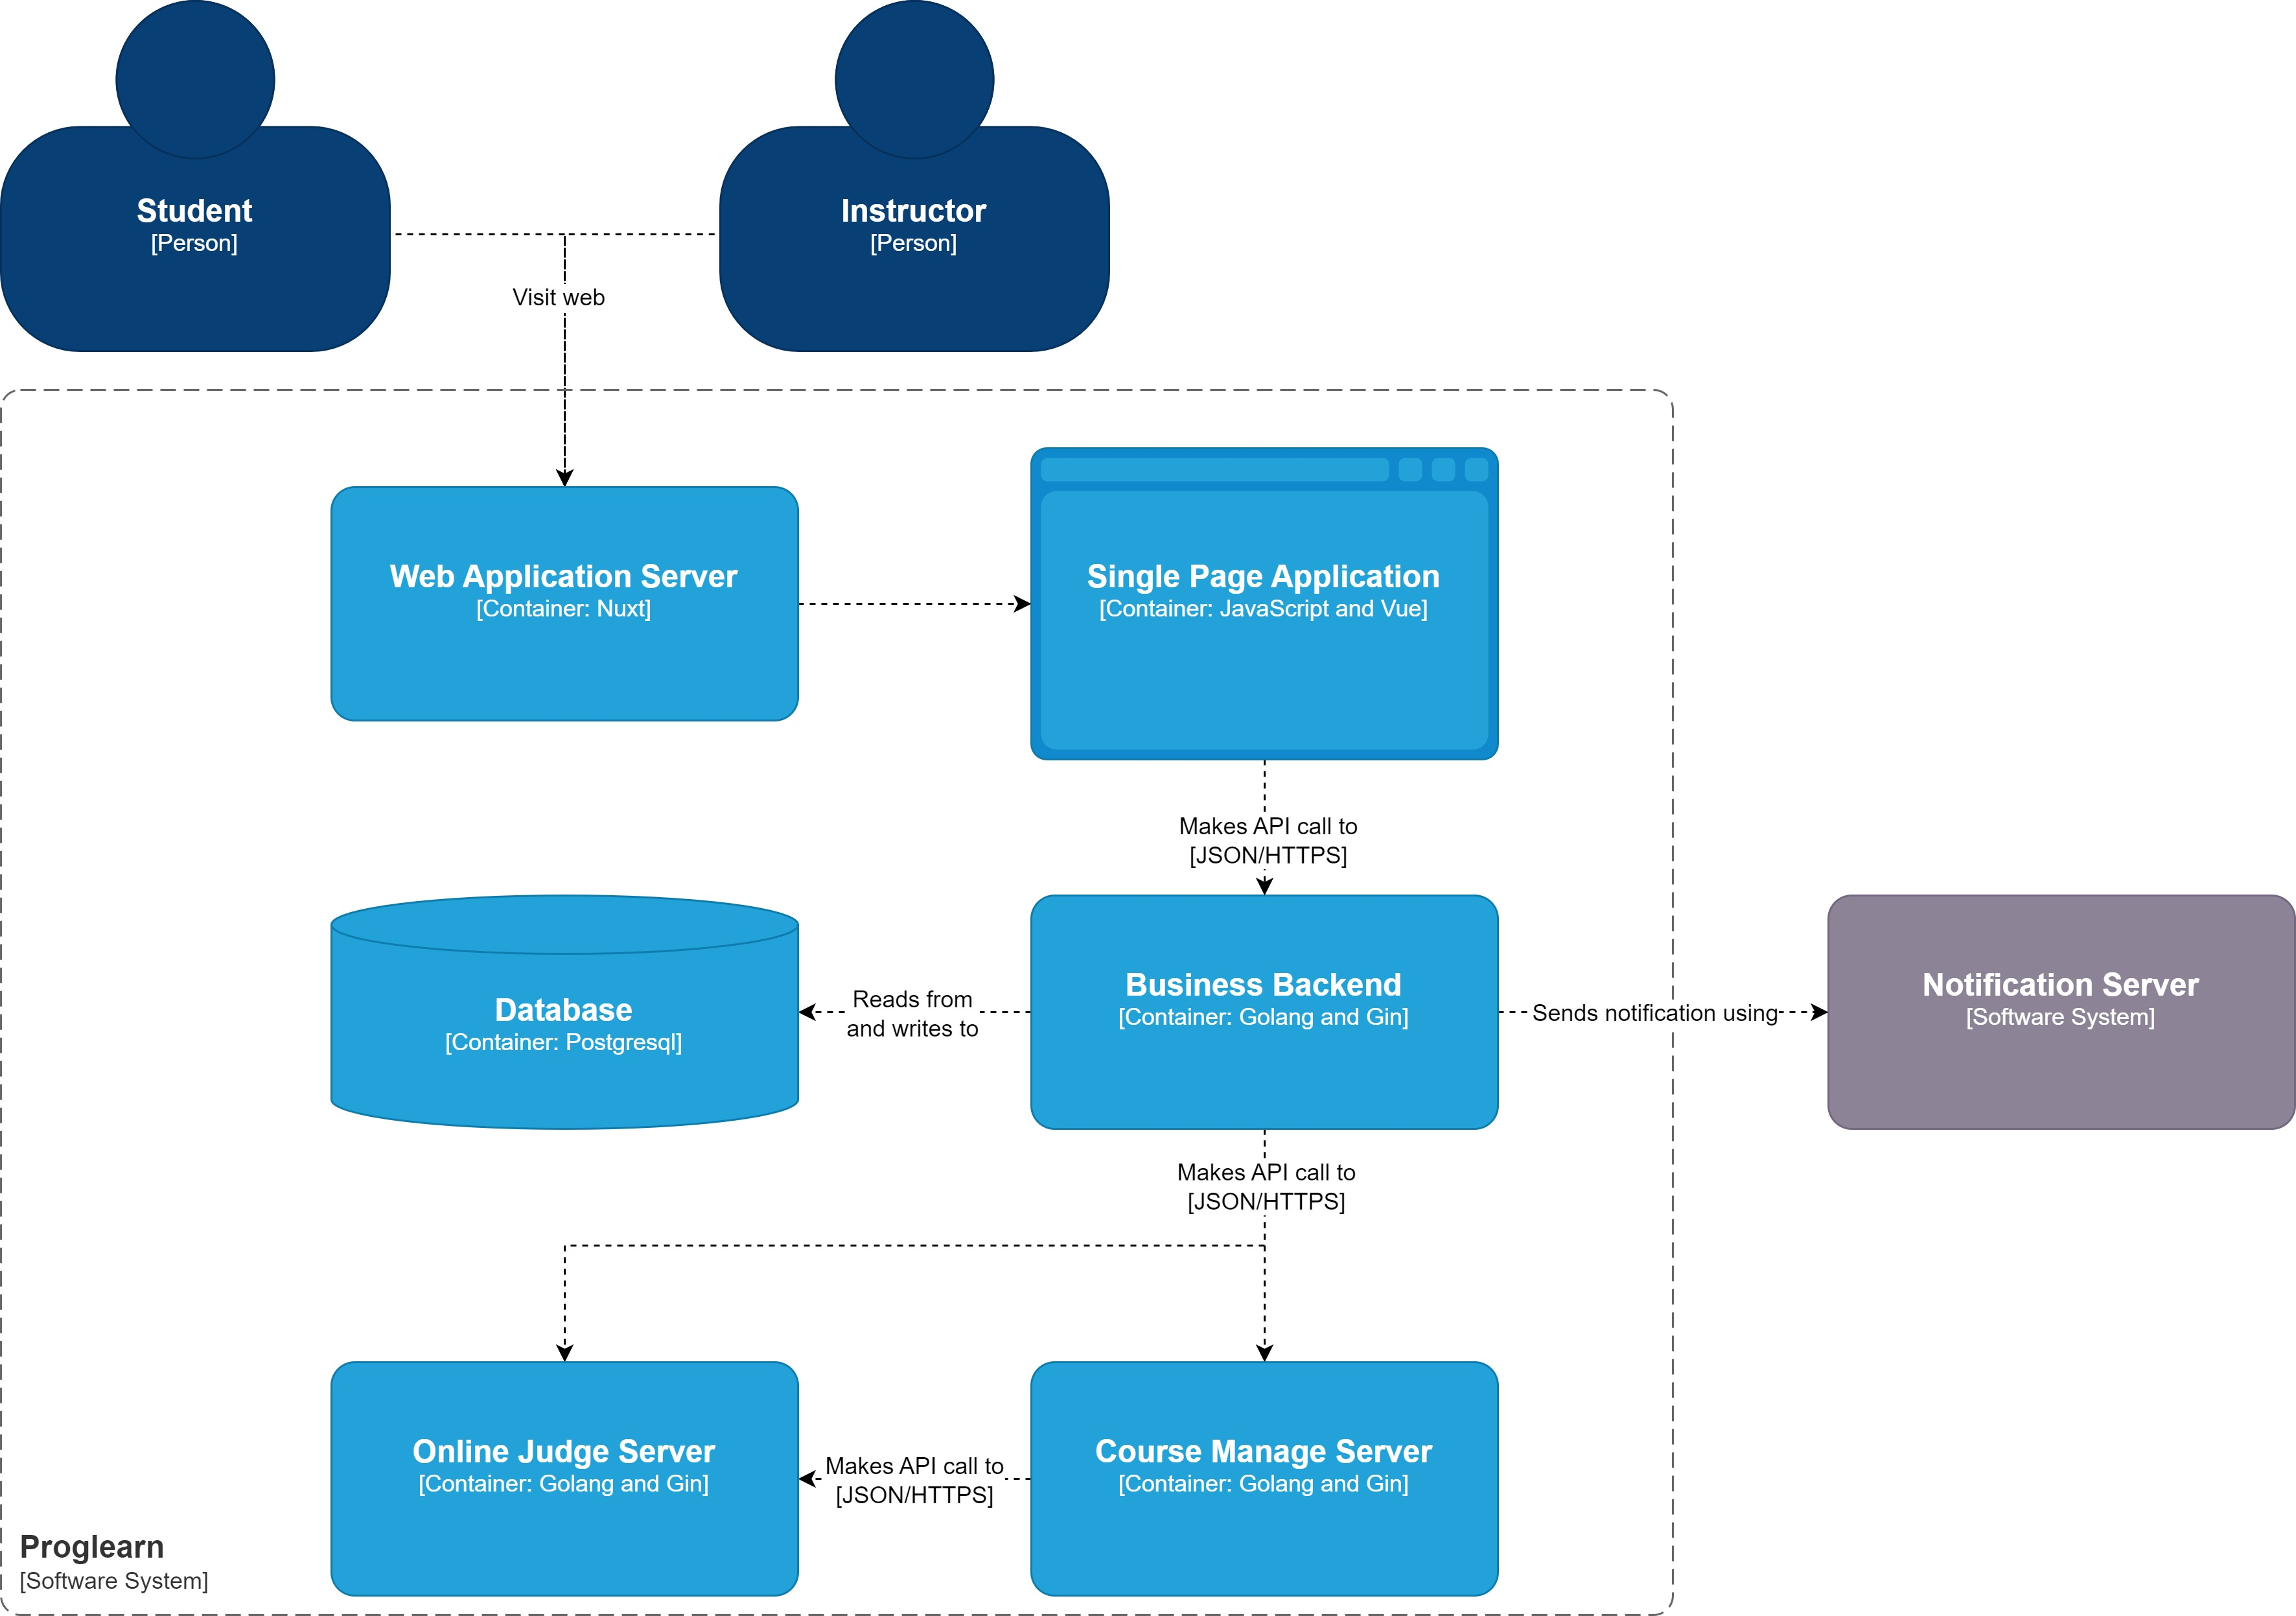
\includegraphics[width=0.65\textwidth]{./img/arc1.jpg}
            }
            \caption{Proglearn 系統架構}
            \label{arc1}            
          \end{subfigure}
          \begin{subfigure}{0.45\linewidth}
            \centering
            \href{https://raw.githubusercontent.com/programingtw/proglearn-plan/main/img/arc2.jpg}{
              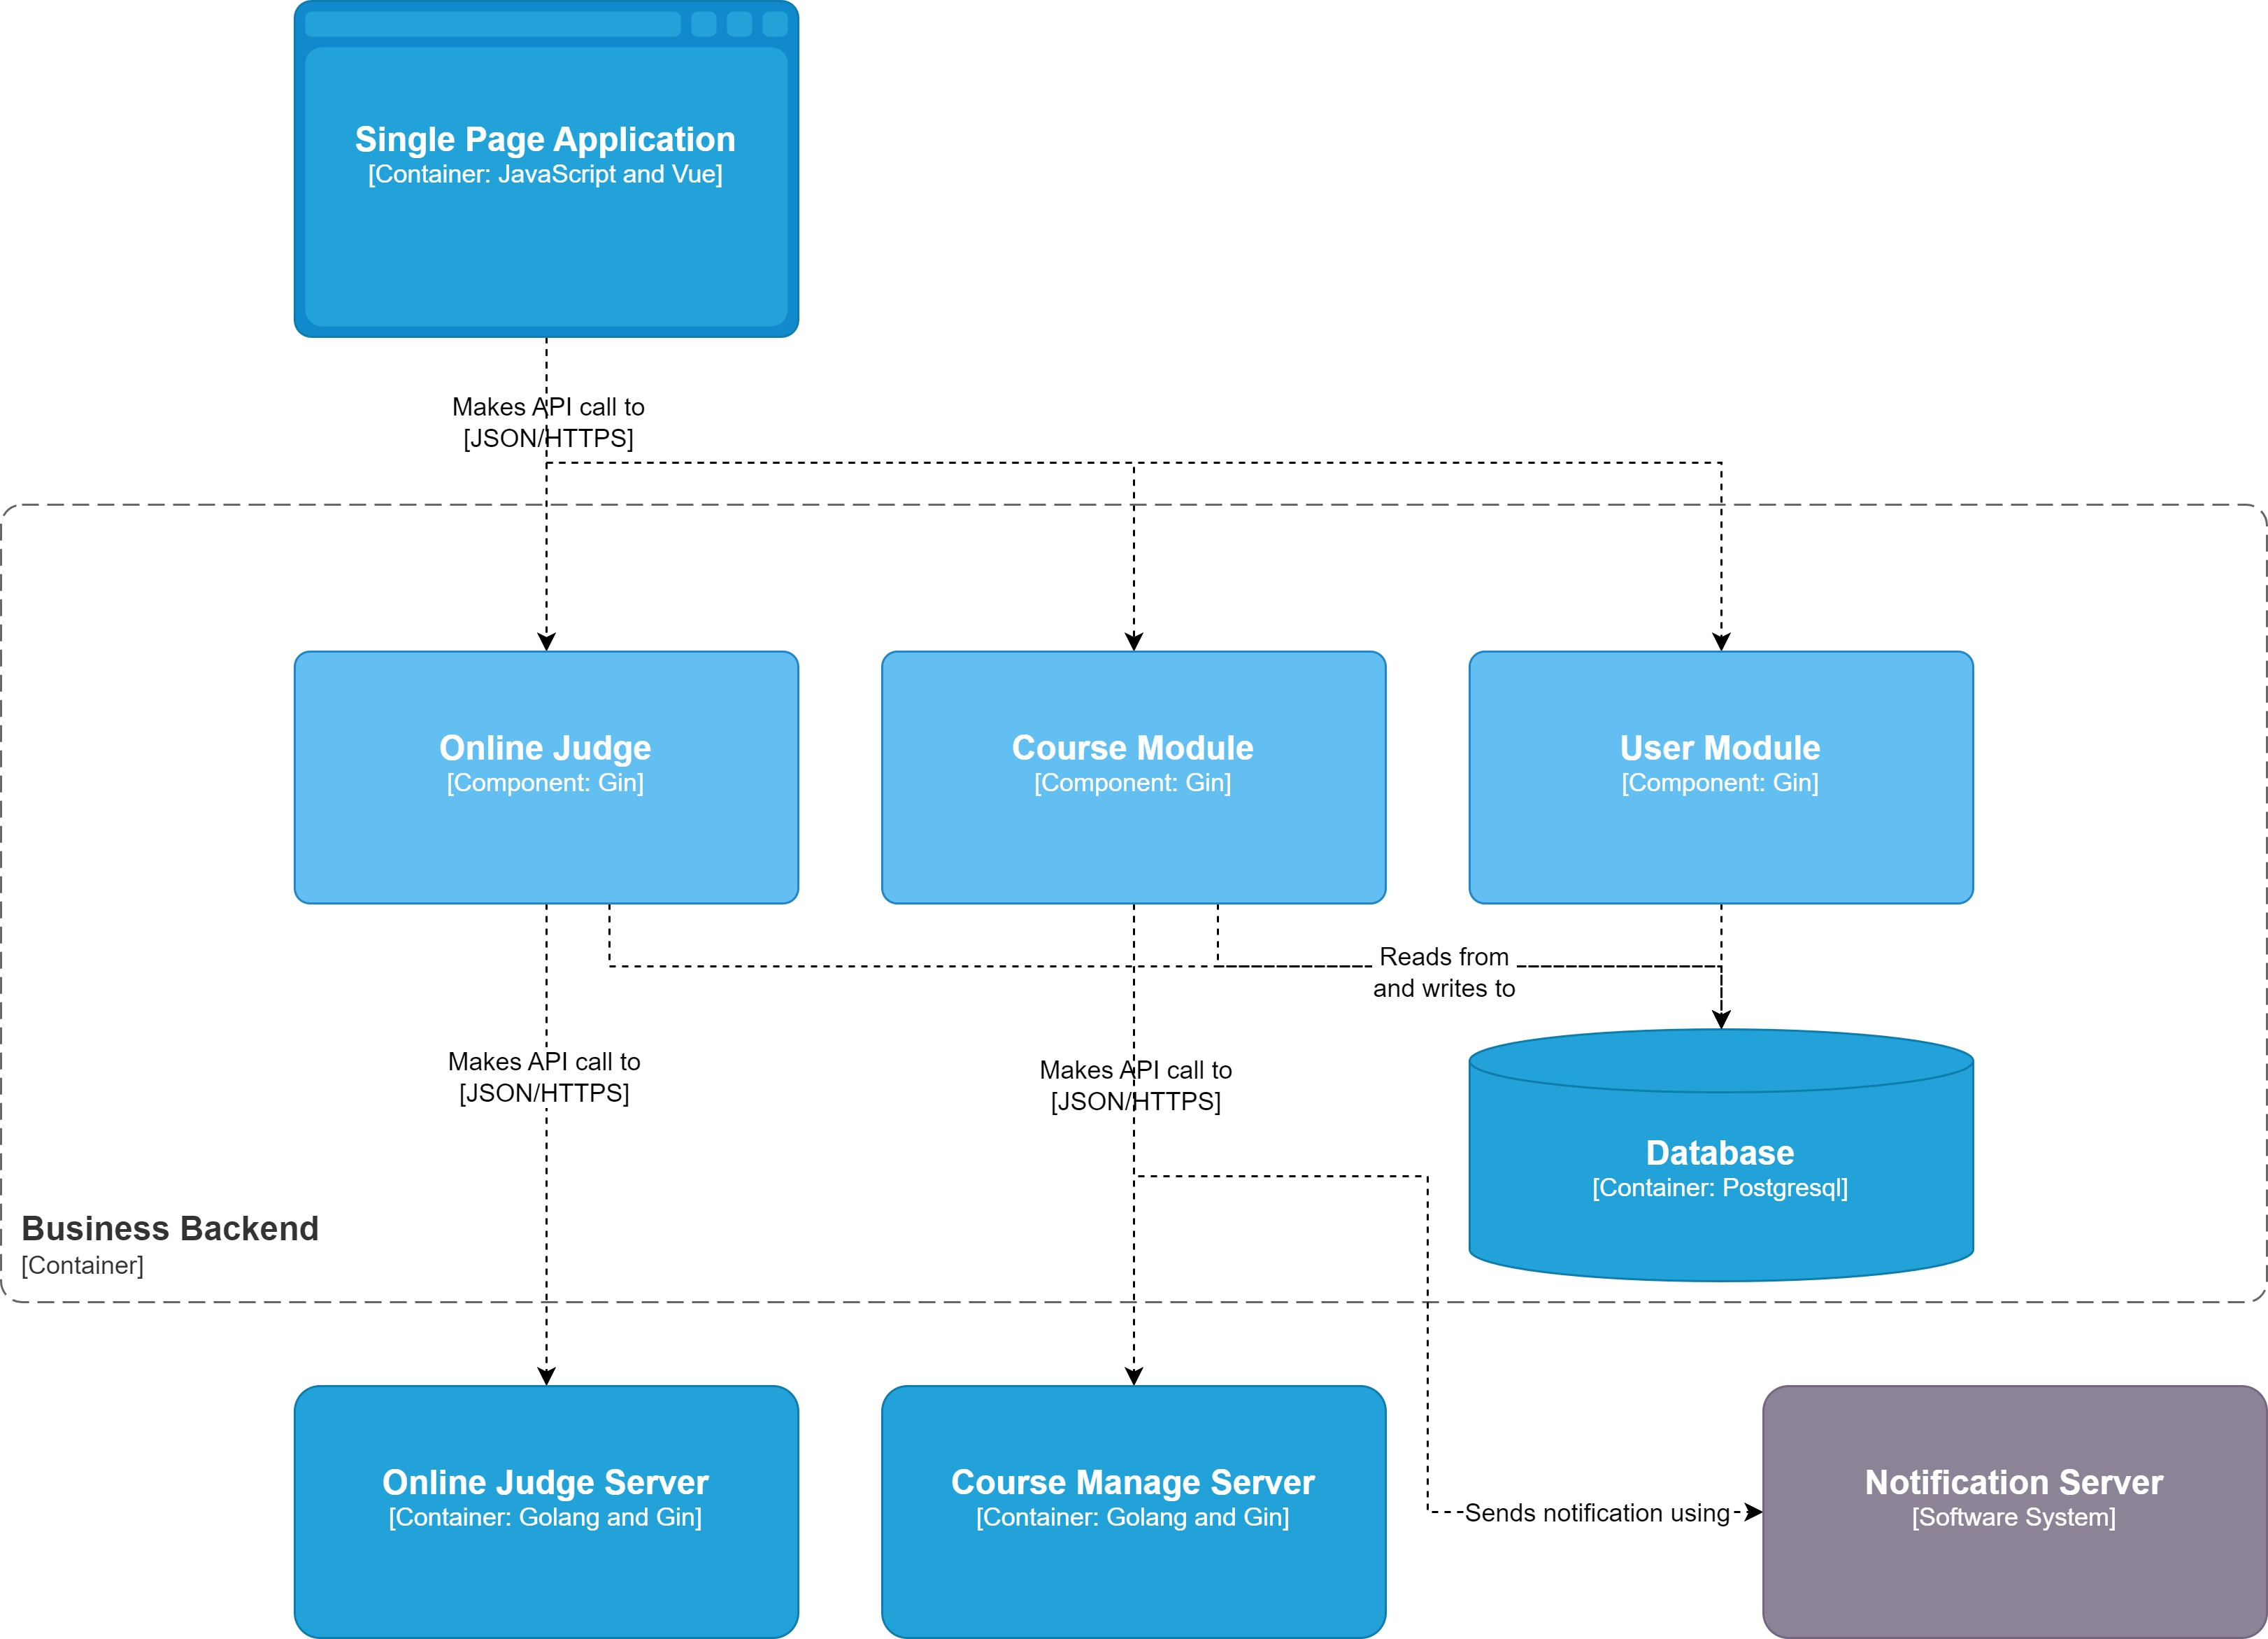
\includegraphics[width=0.65\textwidth]{./img/arc2.jpg}
            }
            \caption{主要後端服務器架構}
            \label{arc2}
          \end{subfigure}
          \bigskip
          \begin{subfigure}{0.45\linewidth}
            \centering
            \href{https://raw.githubusercontent.com/programingtw/proglearn-plan/main/img/arc3.jpg}{
              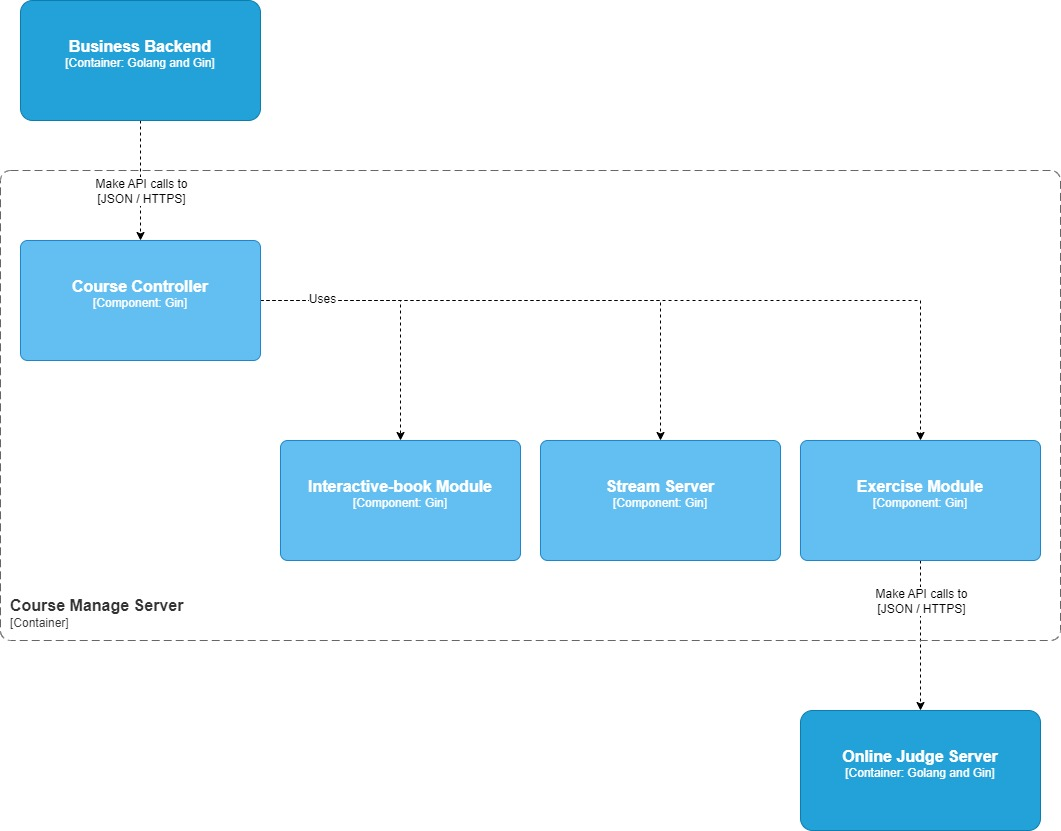
\includegraphics[width=0.65\textwidth]{./img/arc3.jpg}
            }
            \caption{課程管理服務器架構}
            \label{arc3}
          \end{subfigure}
          \begin{subfigure}{0.45\linewidth}
            \centering
            \href{https://raw.githubusercontent.com/programingtw/proglearn-plan/main/img/arc4.jpg}{
              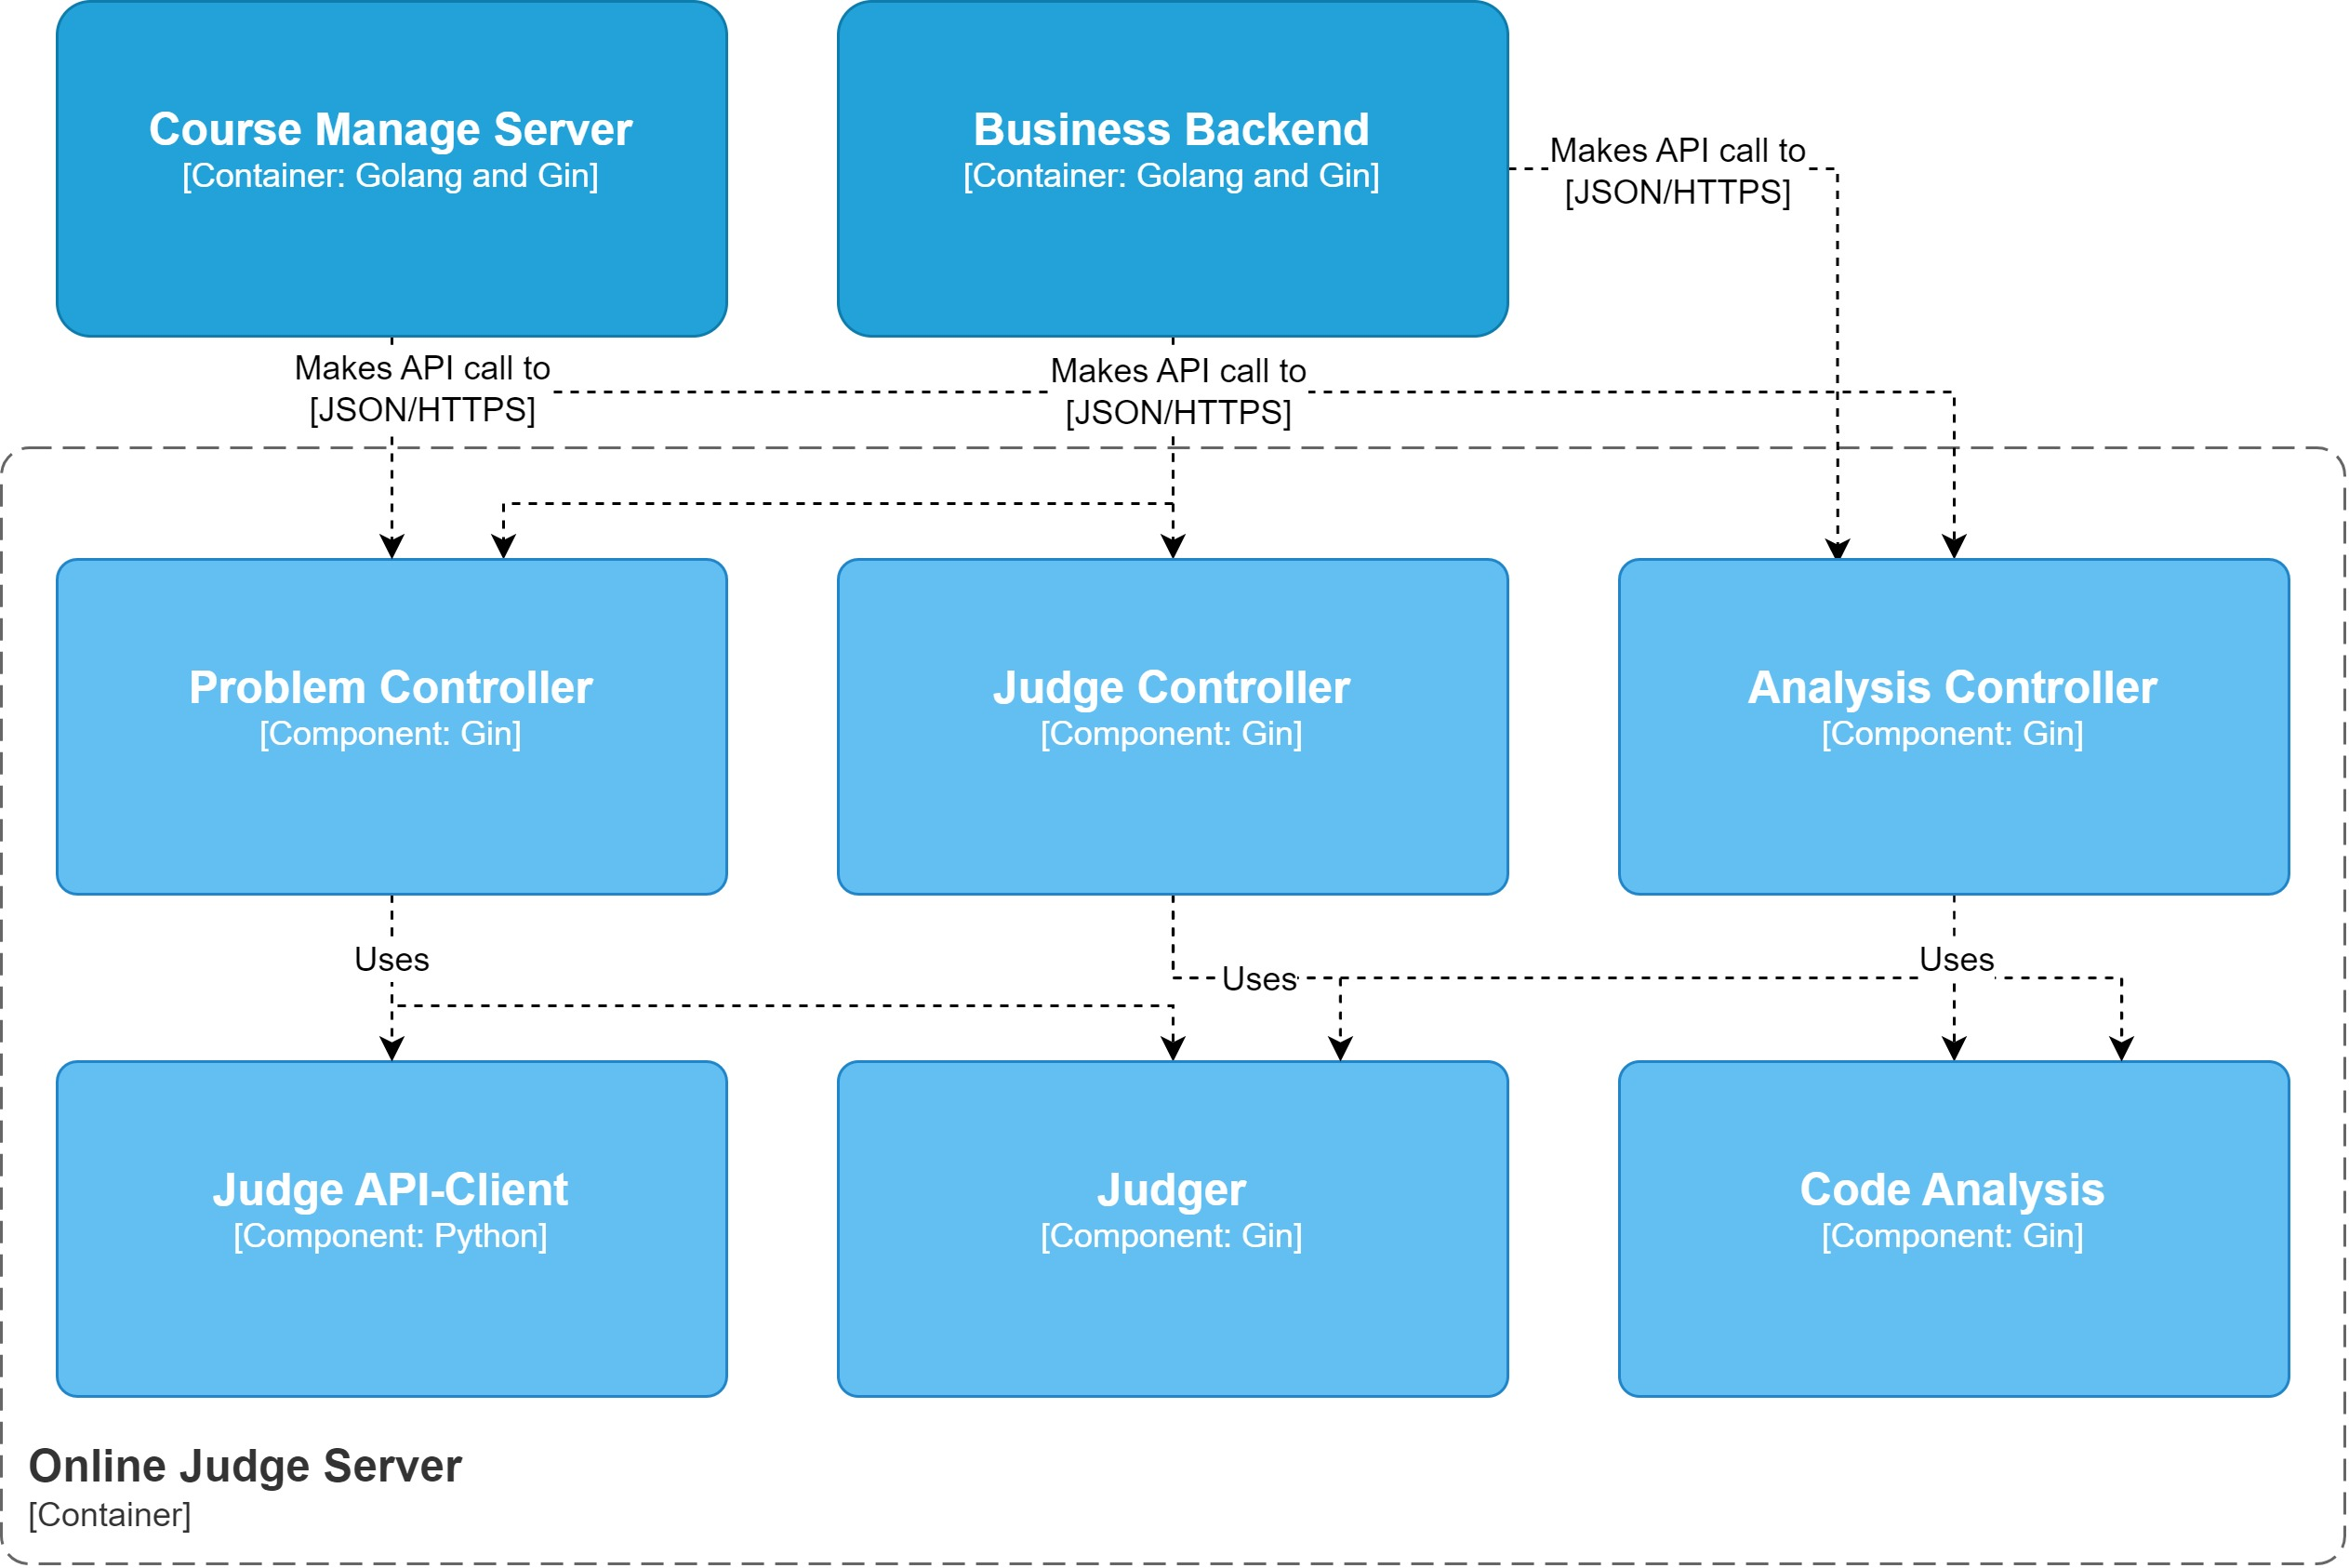
\includegraphics[width=0.65\textwidth]{./img/arc4.jpg}
            }
            \caption{線上解題服務器架構}
            \label{arc4}            
          \end{subfigure}
          \caption{系統架構設計 (點擊可看大圖)}
        \end{figure}
    
        \par 主要後端服務器(如圖\ref{arc2})
          負責處理與管理使用者資料(User Module)、課程模組(Course Module)、題目模組(Online Judge)。
        
        \par 課程管理服務器(如圖\ref{arc3})
          包括影音服務器(Video Server)、投影片模組(Code-Slides Module)、練習模組(Exercise Module)。
          投影片模組將使用 CodeMirror 作為編輯器,並且提供使用 JavaScript 程式碼撰寫投影片。
          前端呈現如圖\ref{arc5},學生能夠同時看到教師的畫面及投影片。
          % 接著使用
        \begin{figure}[H]
          \centering
          \href{https://raw.githubusercontent.com/programingtw/proglearn-plan/main/img/testboard.png}{ 
            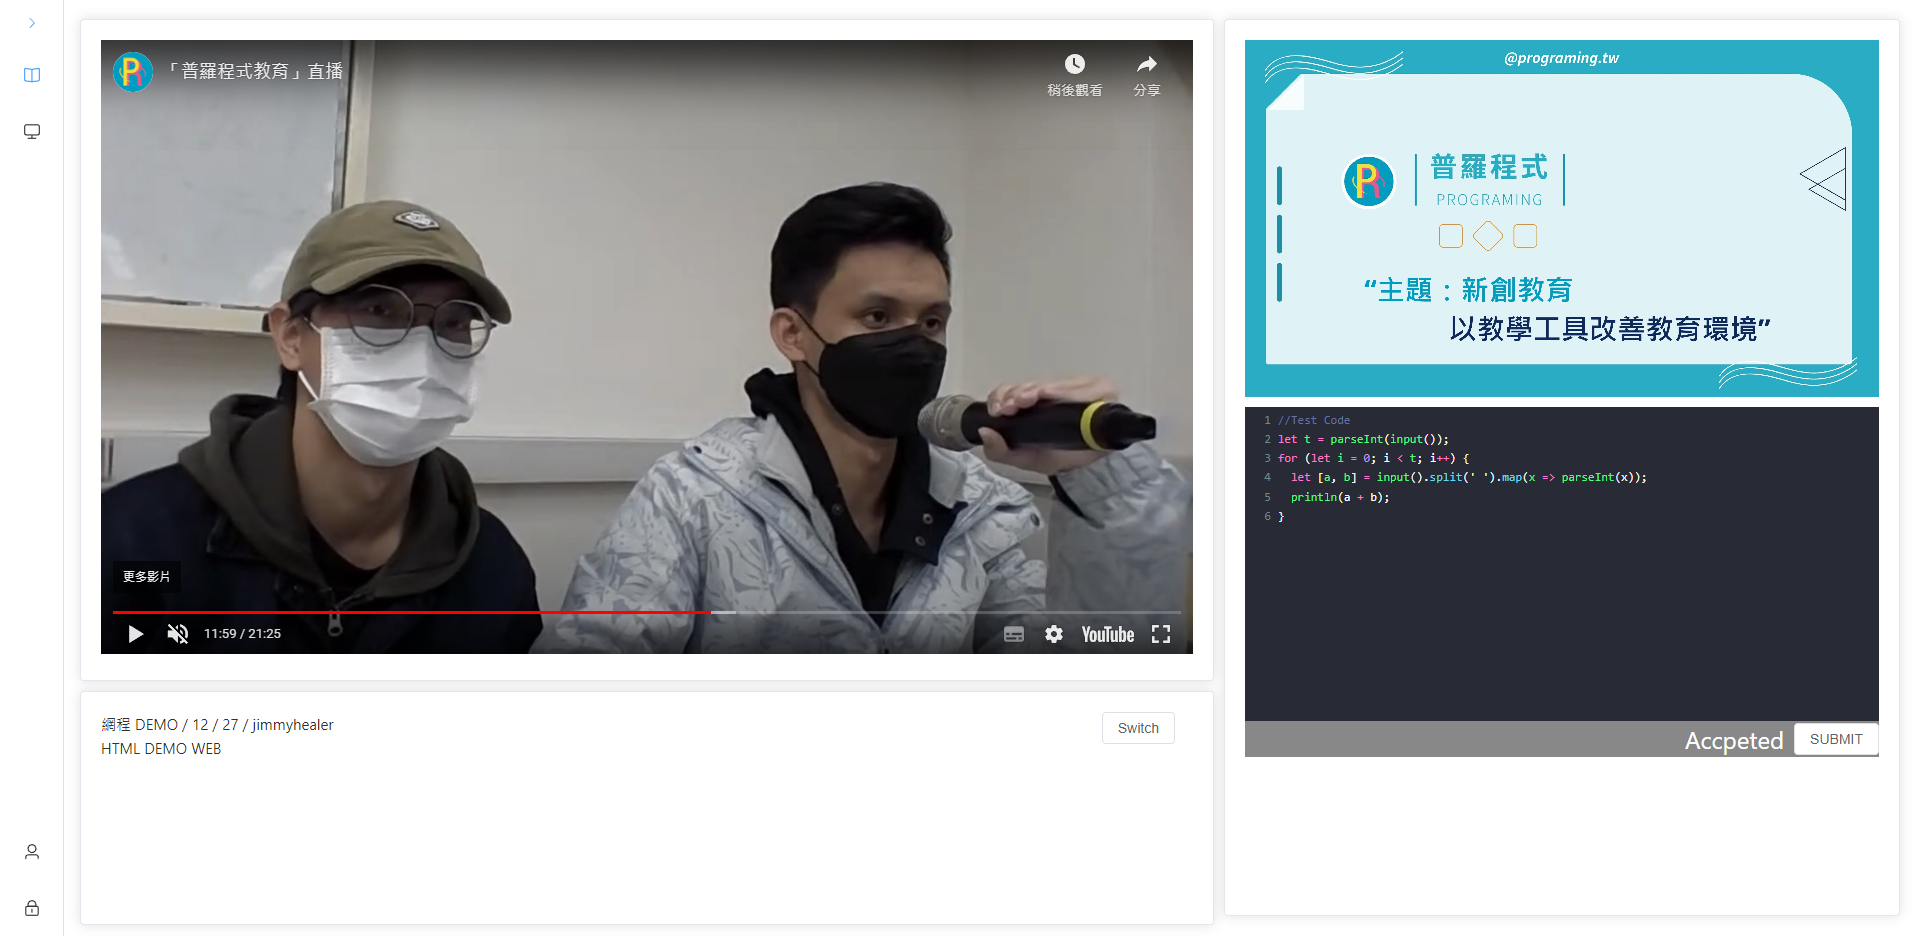
\includegraphics[width=0.5\textwidth]{./img/testboard.png}
          }
          \caption{前端教學頁面示意圖 (點擊可看大圖)}
          \label{arc5}
        \end{figure}
        \par 線上解題服務器(如圖\ref{arc4})
          包括線上題目抓取模組(Judge API-Client)、程式碼批改模組(Judger)、程式碼分析模組(Code Analysis)。
           Judge API-Client 是使用開源專案 api-client \cite{apiclient} 作為線上題目抓取模組,方便教師可以使用現有的題目做修改。
           Judger 是參考開源專案 go-judge \cite{judger1} 、JudgeServer \cite{judger2} 開發出沙盒程式碼執行環境及程式碼批改模組。
           Code Analysis 將採用多標籤辨識模型實現,後續章節將針對此核心技術進行更詳細的說明。
      \item Code Analysis 技術設計
        \begin{enumerate}[label=(\arabic*)]
            \setlength{\parindent}{2em}
            \item 資料準備
              \par 資料來源於 deepmind \footnote{https://www.deepmind.com/} 開發 AlphaCode 所使用的資料集 code\_contests。
              資料集中包含超過 10,000 個題目和程式碼,包含了 AOJ \footnote{Aizu Online Judge, https://judge.u-aizu.ac.jp}
              、Codeforces\footnote{https://codeforces.com}、AtCoder 等。
              資料集中會包含題目和使用者的程式碼,並且將使用 C++、Python、Java 三個常用競賽程式語言作為訓練資料。
              首先我們會先將資料集中的題目依照難度進行分類,將題目分為 5 個等級,分別為 A、B、C、D、E。
              我們計劃整理大約 100 個題目(題目難度分布為 $A:B:C:D:E$ = $4:2:2:1:1$),每個題目都會準備約 100 筆程式碼。
              我們會把這些程式碼分為正確的和錯誤的兩類,比例為 1:9。
            \item 實驗過程
              \par 本研究規劃實驗步驟如圖\ref{ai2}所示。
              首先,我們會將訓練資料集中篩選出 10 題難度為 A 的題目作為初始訓練資料,這些初始訓練資料我們
              會先標記多個錯誤標籤,錯誤標籤包含: 「變數輸入錯誤」(VIE)、「輸出格式錯誤」(OFE)、「演算法時間複雜度過高」(ATH)、
              「變數未初始化」(VAI)、「變數型態錯誤」(VTE)、「演算法錯誤」(AE)、「題意誤解」(PM) 等。
              接著,將這些初始資料切割成 8:2 的比例,其中 8 批資料作為訓練資料,2 批資料作為驗證資料。
              而如圖\ref{ai}所示,會將 題目資訊、程式碼、錯誤標籤 作為輸入,並交給 CodeBERT \footnote{https://github.com/microsoft/CodeBERT} 訓練。
              接著訓練完的模型會把剩餘的訓練資料進行預測,而我們會排序信心分數最低的 20 筆資料進行人工審查與標記,
              並將這些資料加入訓練資料中,並重複上述步驟,直到訓練資料中已審查過的資料都被標記為正確。
              \begin{figure}[H]
                \centering
                \begin{subfigure}{0.3\linewidth}
                  \centering
                  \href{https://raw.githubusercontent.com/programingtw/proglearn-plan/main/img/ai2.jpg}{
                    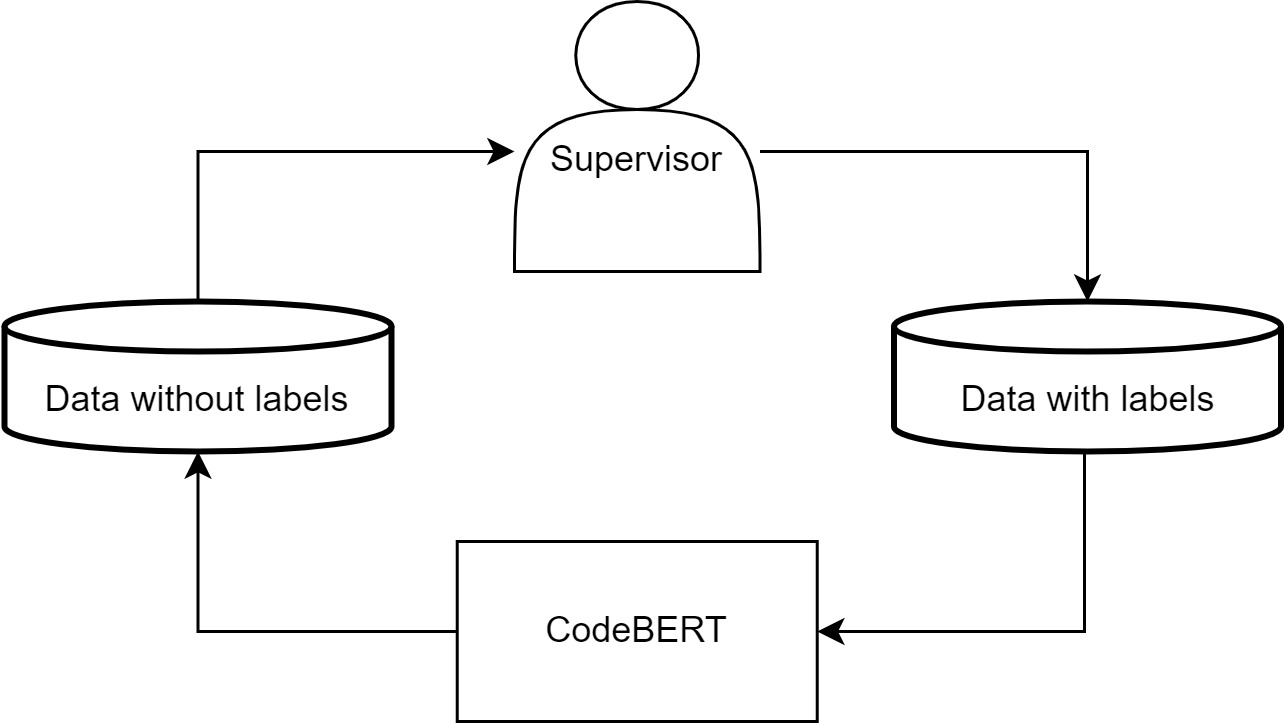
\includegraphics[width=\textwidth]{./img/ai2.jpg}
                  }
                  \caption{主動學習}
                  \label{ai2}
                \end{subfigure}
                \begin{subfigure}{0.3\linewidth}
                  \centering
                  \href{https://raw.githubusercontent.com/programingtw/proglearn-plan/main/img/ai.jpg}{
                    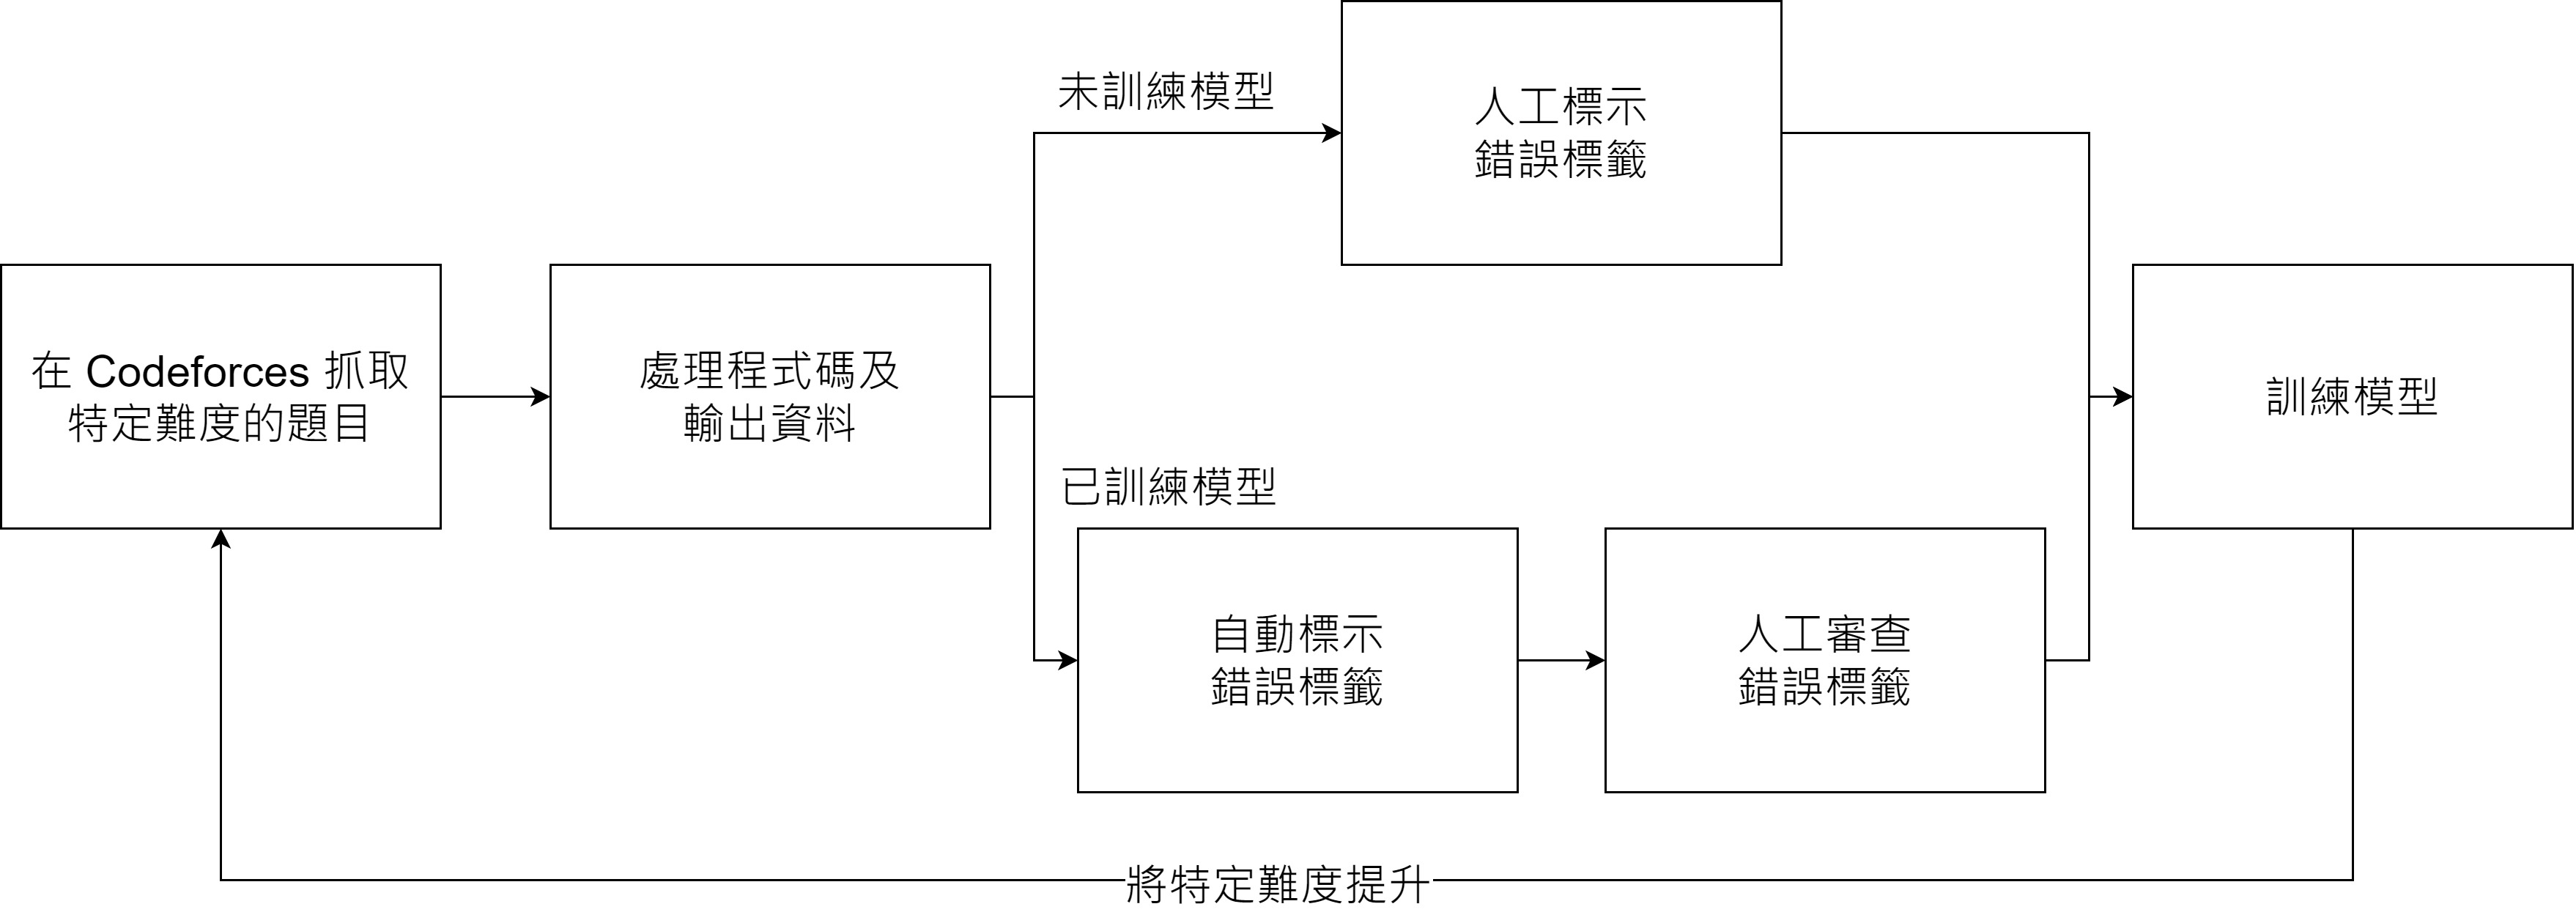
\includegraphics[width=\textwidth]{./img/ai.jpg}
                  }
                  \caption{模型訓練}
                  \label{ai}
                \end{subfigure}
                \caption{AI 訓練實驗步驟 (點擊可看大圖)}
              \end{figure}
            \item 自動反饋使用流程
              \par 本研究規劃的自動反饋使用流程如圖\ref{ai3}所示。
              當學生 (StudentA) 在課堂練習或作業提交程式碼時,會將程式碼交給 Judger 進行批改,
              若是所有的測試資料都通過驗證,Judger 會回傳一個 Accpeted 資訊給結果統計 (Result Statistics),
              若沒有通過驗證,Judger 會回傳一個 Rejected 資訊,並且將程式碼交給 Code Analysis 做錯誤分析。
              接著, Code Analysis 分析後將錯誤標籤給結果統計。
              結果統計會將資訊傳給 StudentA ,並且會將資料統整後傳給教師(Teacher)。
              前端呈現如圖\ref{feedback}所示,教師可以看到某題所有學生的答題情況,掌握學生的學習狀況。
              \begin{figure}[H]
                \centering
                \href{https://raw.githubusercontent.com/programingtw/proglearn-plan/main/img/ai3.jpg}{
                  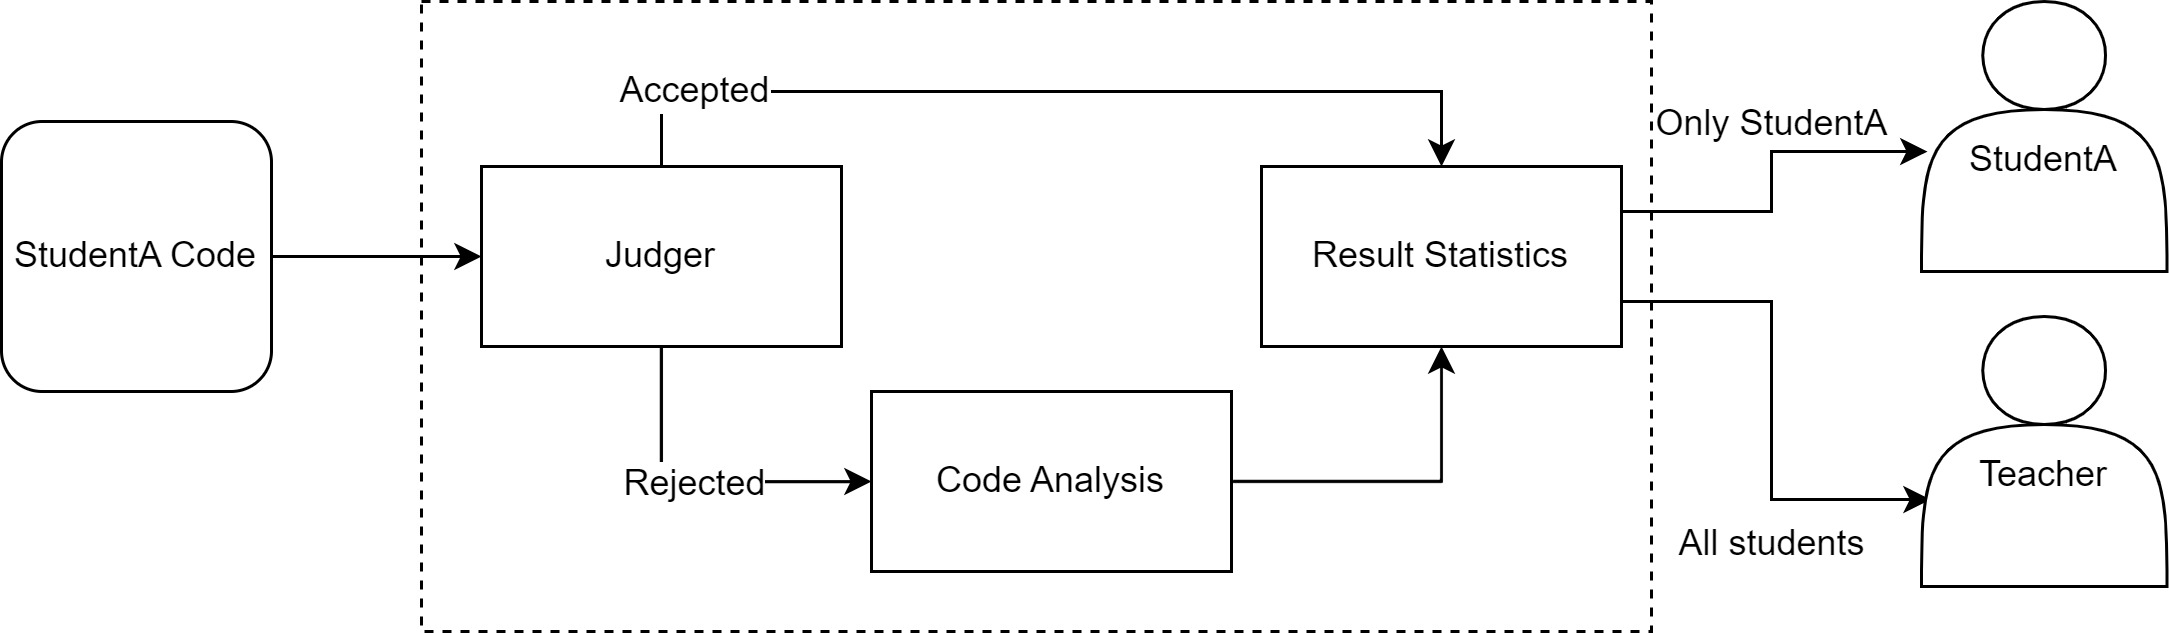
\includegraphics[width=0.7\textwidth]{./img/ai3.jpg}
                }
                \caption{自動反饋使用流程 (點擊可看大圖)}
                \label{ai3}
              \end{figure}
              \begin{figure}[H]
                \centering
                \href{https://raw.githubusercontent.com/programingtw/proglearn-plan/main/img/feedback.png}{
                  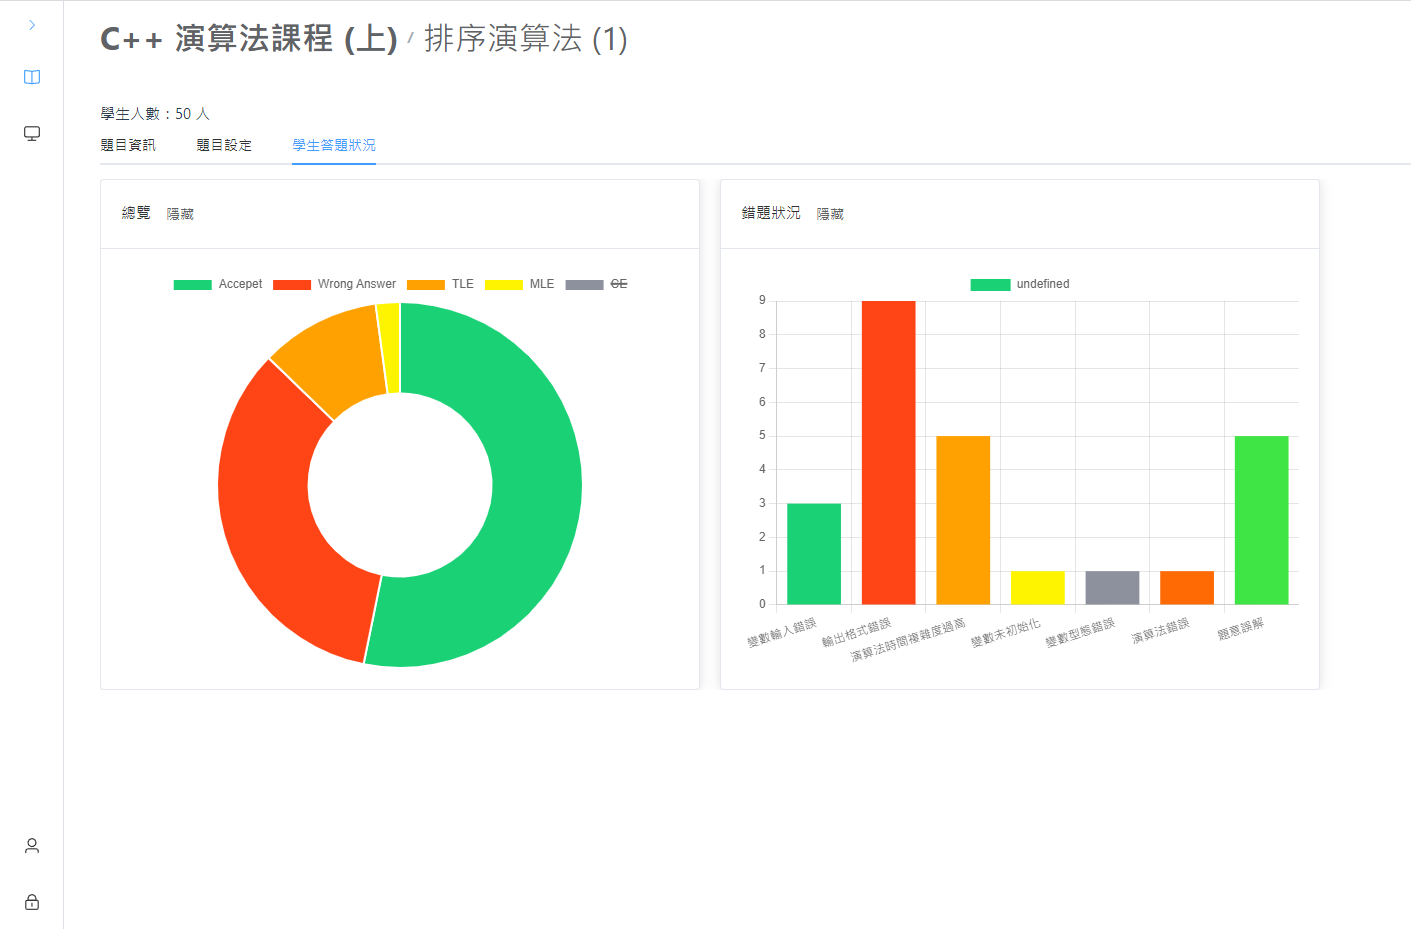
\includegraphics[width=0.7\textwidth]{./img/feedback.png}
                }
                \caption{前端自動反饋介面 (點擊可看大圖)}  
                \label{feedback}
              \end{figure}
        \end{enumerate}

    \end{enumerate}

  \item 預期結果
    \par 最後我們開發出一個整合式教學系統,
    將有以下四點特色:
    \begin{enumerate}
      \item 自動回饋系統能夠節省教師的時間,教師可以快速了解學生的學習進度和弱點,有更多的時間去創造更好的學習環境和教學資源,解決教師在教學與備課的工作量大。
      \item 透過同步練習與課後練習並輔以 AI 自動批改,讓教師能夠快速掌握學生的學習狀況,提高了教學效率。
      \item 互動式簡報模組,可以讓教師與學生之前有更多的互動,讓學生能夠更加主動地參與學習,並且能夠得到及時的回饋和指導。
      \item 整合式系統可以讓教師在同一個平台上創建和管理課程、學生,並能夠快速分析學生的學習狀況,提高了教學效率。
    \end{enumerate}

  \item 參考文獻
    \renewcommand{\section}[2]{}
    \begin{thebibliography}{99}
      \bibitem{ref2} 十二年國民基本教育課程綱要。民112年2月14日,取自:https://www.naer.edu.tw/PageSyllabus?fid=52。
      \bibitem{ref3} 政府資料公開平台(民111年6月29日)。全臺灣各級學校之學生數及畢業生數資料。民112年2月14日,取自:https://data.gov.tw/dataset/31436。
      \bibitem{ref5} 聯合新聞網(民110年3月8日)。中小學資訊教師荒! 多校找自然師兼任遭批不專業。民112年2月14日,取自:https://udn.com/news/story/6885/5303319。
      \bibitem{ref4} 張瑞賓、李建華。"遠距教學常態化問題之探討與建議。" 臺灣教育評論月刊 10.6 (2021): 27-34。
      \bibitem{ref7} 岳修平、梁朝雲。 "綜整學生,教師與教學情境考量的遠距教學預測模型。" 教育資料與圖書館學 52.1 (2015): 33-57+。
      \bibitem{ref8} De Giusti, Armando. "Book review: Policy brief: Education during COVID-19 and beyond." Revista Iberoamericana de Tecnología En Educación y Educación En Tecnología 26 (2020): 110-111.
      \bibitem{ref9} Tumwesige, Josephine. "COVID-19 Educational disruption and response: Rethinking e-Learning in Uganda." University of Cambridge (2020).
      \bibitem{ref10} Santos, Joseline M., and Rowell DR Castro. "Technological Pedagogical content knowledge (TPACK) in action: Application of learning in the classroom by pre-service teachers (PST)." Social Sciences \& Humanities Open 3.1 (2021): 100110.
      \bibitem{ref11} Ratheeswari, K. "Information communication technology in education." Journal of Applied and Advanced research 3.1 (2018): 45-47.
      \bibitem{ref13} Ouya, Samuel, et al. "WebRTC platform proposition as a support to the educational system of universities in a limited Internet connection context." 2015 5th World Congress on Information and Communication Technologies (WICT). IEEE, 2015.
      \bibitem{ref14} Ibrahim, Mohamed, and Osama Al-Shara. "Impact of interactive learning on knowledge retention." Lecture Notes in Computer Science 4558 (2007): 347.
      \bibitem{ref15} Akram, Huma, et al. "Technology integration in higher education during COVID-19: An assessment of online teaching competencies through technological pedagogical content knowledge model." Frontiers in psychology 12 (2021): 736522.
      \bibitem{ref16} Krusche, Stephan, and Andreas Seitz. "Artemis: An automatic assessment management system for interactive learning." Proceedings of the 49th ACM technical symposium on computer science education. 2018.
      \bibitem{ref17} Dong, Yu, Jingyang Hou, and Xuesong Lu. "An intelligent online judge system for programming training." Database Systems for Advanced Applications: 25th International Conference, DASFAA 2020, Jeju, South Korea, September 24–27, 2020, Proceedings, Part III 25. Springer International Publishing, 2020.
      \bibitem{ref18} Delen, Erhan, Jeffrey Liew, and Victor Willson. "Effects of interactivity and instructional scaffolding on learning: Self-regulation in online video-based environments." Computers \& Education 78 (2014): 312-320.
      \bibitem{apiclient} api-client. Available from: https://github.com/online-judge-tools/api-client
      \bibitem{judger1} go-judge. Available from: https://github.com/criyle/go-judge
      \bibitem{judger2} JudgeServer. Available from: https://github.com/helsonxiao/JudgeServer
    \end{thebibliography} 

  \item 需要指導教授內容
    \begin{enumerate}
      \setlength{\parindent}{2em}
      \item 資料收集:學習資料與文獻收集、分析與整理之方法。
      \item 技術分析:學習分析各個功能可能會使用到的相關技術。
      \item 研究方法及步驟:學習利用物件導向軟體工程技術、機器學習技術、
      Web技術來規劃軟體之架構與細部設計。
      \item 系統測試與部署:學習設計不同的測試案例及運用不同的測試方法,以確保本系統之可用性與可靠度,
      並學習如何運用持續整合/部署以及容器技術,進行系統自動化建置與發佈。
    \end{enumerate}
\end{enumerate}
\end{document}